\documentclass[runningheads]{llncs}

\usepackage[T1]{fontenc}
\usepackage[utf8]{inputenc}
\usepackage[british]{babel}
\usepackage{newunicodechar}
\usepackage{xcolor}
\usepackage{minted}
\usepackage{amsmath,amssymb}
\usepackage{mathtools}
\usepackage{graphicx}
\usepackage{pgfplots}
\usepackage{hyperref}
\usepackage{csquotes}
\usepackage{algorithm2e}

\renewcommand\UrlFont{\color{blue}\rmfamily}
\urlstyle{rm}
\SetKw{Kwin}{in}
\def\orcid#1{{\href{http://orcid.org/#1}{\protect\raisebox{-1.25pt}{\protect
\includegraphics{orcid.pdf}}}}}

\newunicodechar{₁}{\ensuremath{_{1}}}
\newunicodechar{₂}{\ensuremath{_{2}}}
\newunicodechar{₃}{\ensuremath{_{3}}}
\newunicodechar{₄}{\ensuremath{_{4}}}
\newunicodechar{₅}{\ensuremath{_{5}}}
\newunicodechar{₆}{\ensuremath{_{6}}}
\newunicodechar{₇}{\ensuremath{_{7}}}
\newunicodechar{₈}{\ensuremath{_{8}}}
\newunicodechar{₉}{\ensuremath{_{9}}}
\newunicodechar{ₙ}{\ensuremath{_{n}}}
\newunicodechar{ₘ}{\ensuremath{_{m}}}
\newunicodechar{ᵢ}{\ensuremath{_{i}}}
\newunicodechar{ⱼ}{\ensuremath{_{j}}}
\newunicodechar{ₗ}{\ensuremath{_{l}}}
\newunicodechar{ₖ}{\ensuremath{_{k}}}
\newunicodechar{α}{\ensuremath{\alpha}}
\newunicodechar{σ}{\ensuremath{\sigma}}
\newunicodechar{τ}{\ensuremath{\tau}}
\newunicodechar{λ}{\ensuremath{\lambda}}
\newunicodechar{μ}{\ensuremath{\mu}}
\newunicodechar{η}{\ensuremath{\eta}}
\newunicodechar{Γ}{\ensuremath{\Gamma}}
\newunicodechar{Δ}{\ensuremath{\Delta}}
\newunicodechar{Φ}{\ensuremath{\Phi}}
\newunicodechar{Ψ}{\ensuremath{\Psi}}
\newunicodechar{Ω}{\ensuremath{\Omega}}
\newunicodechar{∈}{\ensuremath{\in}}
\newunicodechar{∉}{\ensuremath{\notin}}
\newunicodechar{≡}{\ensuremath{\equiv}}
\newunicodechar{≢}{\ensuremath{\nequiv}}
\newunicodechar{≠}{\ensuremath{\neq}}
\newunicodechar{≤}{\ensuremath{\leq}}
\newunicodechar{≔}{\ensuremath{\coloneq}}
\newunicodechar{∧}{\ensuremath{\land}}
\newunicodechar{∨}{\ensuremath{\lor}}
\newunicodechar{∪}{\ensuremath{\cup}}
\newunicodechar{∩}{\ensuremath{\cap}}
\newunicodechar{⊆}{\ensuremath{\subseteq}}
\newunicodechar{⋃}{\ensuremath{\bigcup}}
\newunicodechar{→}{\ensuremath{\rightarrow}}
\newunicodechar{↔}{\ensuremath{\leftrightarrow}}
\newunicodechar{↦}{\ensuremath{\mapsto}}
\newunicodechar{⊢}{\ensuremath{\vdash}}
\newunicodechar{∅}{\ensuremath{\emptyset}}
\newunicodechar{∷}{\ensuremath{\mathbin{::}}}
\newunicodechar{⇒}{\ensuremath{\Rightarrow}}
\newunicodechar{ℕ}{\ensuremath{\mathbb{N}}}
\newunicodechar{⟨}{\ensuremath{\langle}}
\newunicodechar{⟩}{\ensuremath{\rangle}}
\newunicodechar{⊤}{\ensuremath{\top}}
\newunicodechar{⊥}{\ensuremath{\bot}}
\newunicodechar{×}{\ensuremath{\times}}

\newtheorem{lem}{Lemma}

\setminted[lean4]{extrakeywords={aesop cases add aesop? intro simp simp_all only split apply on_goal next rename_i safe unsafe norm constructors forward destruct norm_num done add_aesop_rules rfl subst ext}}
\newmintinline[lean]{lean4}{bgcolor={},ignorelexererrors=true}
\newminted[leancode]{lean4}{bgcolor={},ignorelexererrors=true,fontsize=\footnotesize,autogobble}
\BeforeBeginEnvironment{leancode}{\begin{tcolorbox}}
\AfterEndEnvironment{leancode}{\end{tcolorbox}}
\usemintedstyle{xcode}

\newcommand{\xcom}[1]{{\color{cyan}{Xavier: #1}} }
\newcommand{\jcom}[1]{{\color{orange}{Jannis: #1}} }

\newcommand{\Lam}[2]{\ensuremath{\lambda\, #1,\; #2}}
\newcommand{\All}[2]{\ensuremath{\forall\, #1,\; #2}}
\newcommand{\mvar}[1]{\ensuremath{?#1}}
\newcommand{\Prop}{\ensuremath{\mathrm{Prop}}}
\newcommand{\vars}{\ensuremath{\mathrm{vars}}}
\newcommand{\dom}{\ensuremath{\mathrm{dom}}}
\newcommand{\sub}{\ensuremath{\mathrm{sub}}}
\newcommand{\lvl}{\ensuremath{\mathrm{lvl}}}
\newcommand{\Rules}{\ensuremath{\mathcal{R}}}
\newcommand{\Hyps}{\ensuremath{\mathcal{H}}}
\newcommand{\States}{\ensuremath{\mathcal{S}}}
\newcommand{\CMatches}{\ensuremath{\mathcal{C}}}
\newcommand{\addHyp}{\ensuremath{\mathrm{addHyp}}}
\newcommand{\delHyp}{\ensuremath{\mathrm{delHyp}}}
\newcommand{\powerset}{\ensuremath{\mathbb{P}}}

\begin{document}

\title{Incremental Forward Reasoning for White-Box~Proof~Search}

%\titlerunning{Abbreviated paper title}
% If the paper title is too long for the running head, you can set
% an abbreviated paper title here

\author{Jannis Limperg\orcid{0000-0002-8861-5231} \and
  Xavier Généreux\orcid{0000-0003-4952-9557}}

\authorrunning{J.~Limperg and X.~Généreux}
\institute{Ludwig-Maximilians-Universität München, Munich, Germany\\
\email{\{jannis.limperg,xavier.genereux\}@lmu.de}}

\maketitle

\begin{abstract}
  Several proof assistants provide automation tactics based on tableau-style tree search, such as Isabelle's and Rocq's auto and Lean's Aesop.
  In this setting we consider \emph{forward rules}, which apply a given theorem, say, $A → B → C$, to any goal containing hypotheses $A$ and $B$, adding $C$ as a new hypothesis.
  When treated naively, such rules are tried on every goal encountered during the search, leading to repeated unifications of premises $A$ and $B$ with the hypotheses of each goal.
  We present an approach to forward rules that avoids some of this repeated work by taking advantage of similarities between successive goals.
  For each goal, we cache partial applications of forward rules in a custom data structure, the \emph{partial match state}, which enables efficient updates.
  Our technique is compatible with any search strategy and most logics.
  It has been implemented in Aesop.

  \keywords{Forward Reasoning \and Forward Chaining \and Tactics \and Interactive Theorem Proving.}
\end{abstract}

\section{Introduction}

In many proof assistants, simple automation tactics based on tableau-style tree search play a substantial role in practice: Isabelle's (TODO ref) and Rocq's (TODO ref) auto, ACL2's (TODO ref) waterfall, PVS's (TODO ref) grind, Lean's (TODO ref) Aesop (TODO ref), etc.
These tactics operate on \emph{goals} $Γ ⊢ A$, where the \emph{local context} $Γ$ is a list of assumptions and $A$ is the proposition to be proved.
Faced with an initial goal, the tactics try various user-specified \emph{rules}, which correspond to admissible inferences in the prover's logic.
A successful rule reduces the current goal to zero or more subgoals, which are solved recursively until either a full proof is found or no rule applies to any open goal or the search times out.

Typical rules would be the $∧$-introduction lemma $A → B → A ∧ B$, which, when applied backwards, reduces a goal $Γ ⊢ A ∧ B$ to subgoals $Γ ⊢ A$ and $Γ ⊢ B$; or left $∨$-introduction, which reduces $Γ ⊢ A ∨ B$ to $Γ ⊢ A$.
Such \emph{backward rules} are the most common rule type, but most search tactics allow users to use any tactic as a rule.
These rule tactics can output arbitrary subgoals, subject only to the condition that proofs of the returned subgoals can be assembled into a proof of the goal on which the rule was run.

ACL2 and Aesop additionally provide special support for \emph{forward rules}.
Given, for example, the transitivity lemma $\All{x~y~z}{x < y → y < z → x < z}$, a forward rule run on the goal $a < b,\, b < c ⊢ A$ produces the single subgoal $a < b,\, b < c,\, a < c ⊢ A$.
Hence forward rules can be used to establish additional facts that may be relevant for other rules.
For example, the Aeneas project (TODO ref) uses Aesop's forward rules \jcom{(ensure that this is accurate)} in its proof automation to establish facts that are later used by an arithmetic decision procedure.

However, Aesop's (and ACL2's) support for forward rules was, until recently, quite basic.
In particular, each forward rule was tried on each goal separately (subject to pre-filtering by a discrimination tree (TODO ref) index).
This is wasteful since in practice, many rules produce subgoals with a similar---or even the same---local context as the initial goal.
For example, the ∧-introduction rule affects only the goal's target, not its context.
Still, all forward rules applied to the initial $Γ ⊢ A ∧ B$ would be tried again on the subgoals $Γ ⊢ A$ and $Γ ⊢ B$, with predictably little effect.

In this paper, we present an alternative way to apply forward rules that addresses this issue.
The central idea is to remember, for each goal $Γ ⊢ A$, which forward rules can be partially applied to which sets of hypotheses.
When a non-forward rule then generates subgoals $Δ₁ ⊢ A₁$, \dots, $Δₙ ⊢ Aₙ$, the new local contexts $Δᵢ$ are likely similar to $Γ$.
Hence it is generally cheaper (and often much cheaper) to start with the partial matches for $Γ$ and update them for each of the $Δᵢ$.
The update first deletes partial matches that include hypotheses no longer present in $Δᵢ$.
Afterwards it adds new partial matches for the hypotheses that are new in $Δᵢ$, extending the existing partial matches for a rule if the new hypothesis is compatible with them.
Whenever this process produces a full match---i.e., all premises of a forward rule are satisfied by a set of hypothesis in $Δᵢ$---the rule is applied and adds a corresponding new hypothesis to $Δᵢ$.
Our main contribution is a data structure, the \emph{partial match state}, that organises the partial matches in such a way that the update can be done efficiently.

In addition to supporting such \emph{incremental} forward reasoning, the partial match state satisfies two other desiderata:
\begin{itemize}
  \item It is \emph{persistent}, i.e.\ partial match states for parent and child goals share much of their structure.
        This is desirable since Aesop supports search strategies other than depth-first search and must therefore keep all goals encountered during the search, along with their partial match states, in memory.
  \item It reduces the number of \emph{unifications} performed when matching hypotheses against rule premises.
        In dependent type theory, unification happens up to definitional equality, which makes it quite expensive.
        We therefore want to avoid redundant unifications.
\end{itemize}

Our evaluation (Sec.~\ref{sec:evaluation}) shows that this new implementation of forward reasoning in Aesop substantially outperforms the previous, naive implementation in some (though not all) cases.
The implementation, the benchmarks we used and the full evaluation data are available in a supplement to this paper (TODO ref).
Mainline Aesop already uses the new implementation by default (TODO true?).

\section{Preliminaries}

We first introduce some terminology for matches and for forward rules (which we identify with their underlying lemmas).
Our foundation in this paper is dependent type theory, but our technique can be adapted to other logics.

Given a lemma $\All{(x₁ : A₁) \dots (xₙ : Aₙ)}{B}$, the $xᵢ$ are \emph{premises} and $B$ is the lemma's \emph{conclusion}.
The type $Aᵢ$ of the $i$-th premise may depend on (i.e., refer to) any premise $xⱼ$ with $j < i$.
Implication $A → B$ is an abbreviation for $\All{x : A}{B}$ where $B$ does not depend on $x$.
Propositions are (certain) types and we do not distinguish between the two concepts.

Premises on which a later premise depends are \emph{variables}.
All other premises are \emph{input premises}.
For example, the lemma $\All{x~y~z}{x < y → y < z → x < z}$ has variables $x, y, z$ and (unnamed) input premises of types $x < y$ and $y < z$.
If a variable occurs in at least two premises, like $y$ above, it is \emph{shared}.

For a lemma with $n$ input premises, we assign to each input premise a unique number between $1$ and $n$.
This is the premise's \emph{slot}, which we often identify with the premise itself.
For now, we assume that the input premises are numbered consecutively, so in the above example slot 1 has type $x < y$ and slot 2 has type $y < z$.
The \emph{shared variables of slot $i$}, $\vars(i)$ are those variables that appear in the type of $i$ and also in at least one type of a slot $j < i$.

If $h : A$ is a hypothesis in the local context of a goal and $A$ unifies with the type $B$ of slot $i$, we say that $h$ \emph{matches} $i$.
Unification induces a substitution $σ$ (with $\dom(σ) ⊆ \vars(i)$) such that $A[σ]$ is definitionally equal to $B[σ]$; we call this substitution $\sub_{i}(h)$.
For now we do not specify exactly what \enquote{unifies} means; see Sec.~\ref{sec:unification}.

A \textit{match} $M$ for a given rule $r$ is a partial map from slots of $r$ to hypotheses.
The map must satisfy the following conditions:
\begin{enumerate}
  \item\label{cond:match:matches} For each slot $i ∈ \dom(M)$, the hypothesis $M(i)$ matches $i$.
  \item\label{cond:match:compat} For all slots $i,j ∈ \dom(M)$, the substitutions $\sub_{i}(M(i))$ and $\sub_{j}(M(j))$ are \emph{compatible}.
        This means that for each variable $x ∈ \dom(\sub_{i}(M(i))) ∩ \dom(\sub_{j}(M(j)))$ we have $\sub_{i}(M(i))(x) = \sub_{j}(M(j))(x)$, i.e.\ the substitutions agree on all common variables.
  \item\label{cond:match:closed} $M$ is \emph{downward-closed}: if $i ∈ \dom(M)$, then for any slot $j < i$ of $r$ we also have $j ∈ \dom(M)$.
\end{enumerate}
The \emph{substitution of a match $M$}, $\sub(M)$, is the union of the substitutions induced by the hypotheses in $M$, i.e. $\sub(M) ≔ ⋃_{i ∈ \dom(M)}\sub_{i}(M(i))$.
This is well-defined by requirement~\ref{cond:match:compat}.
The \textit{level of a match $M$}, $\lvl(M)$, is the maximal $i$ such that $i ∈ \dom(M)$.
A match for rule $r$ is \textit{complete} if $i ∈ \dom(M)$ for every slot $i$ of $r$, and \emph{partial} otherwise.

A partial match $M$ for rule $r$ corresponds to a partial application of the rule to the terms given in $\sub(M)$.
The application is type-correct by requirements~\ref{cond:match:matches} and~\ref{cond:match:compat}.
If $M$ is complete, then $\sub(M)$ contains a term for every slot and every variable---hence for every premise---of $r$ and we have a full application.

\section{Naive Forward Reasoning}

Prior to this work, Aesop used what we call naive forward reasoning (TODO ref).
This approach treats a forward rule essentially like any other Aesop rule.
Hence, given a goal $h₁ : T₁,\, \dots, hₙ : Tₙ ⊢ U$, we first query an index to determine which rules might apply to the goal.
For forward rules, this index stores the type of the last premise (since later premises tend to be more specific).
The index is queried for each $Tᵢ$, yielding a set of rules that have a premise which likely unifies with at least one hypothesis.
Of these rules and any non-forward rules selected in a similar way, we select the highest-priority one.

If the selected rule is a forward rule $r : \All{(x₁ : A₁) \dots (xₘ : Aₘ)}{B}$, we first unify $Aₘ$ with one of the candidate hypotheses determined by the index.
If successful, this results in a substitution $σ$ whose domain contains $xₘ$ and any variables occurring in $Aₘ$.
We then proceed to unify $A_{m-1}[σ]$ with the type of each hypothesis in the context, etc., until we have found a complete match for $r$ (skipping premises already determined by $σ$).
If a premise type $A_{i}[σ]$ does not unify with any hypothesis type, we backtrack and consider other potential matching hypotheses for $A_{i+1}$.
This may lead to a different substitution $τ$ and therefore to matching hypotheses for $A_{i}[τ]$.

If this process yields one or more full applications $r~a₁ \dots aₘ$, we add $B[x₁ ↦ a₁, \dots, xₘ ↦ aₘ]$ as a new hypothesis unless a hypothesis of this type is already present in the context.

\jcom{Add example?}

This approach is efficient when the last premise of a rule is not present in the context since the rule is then never run.
If the last premise is present, however, we perform a large number of unifications between premises and hypotheses.
Furthermore, these unifications are repeated when we proceed to another goal with a similar context.
In particular, the contexts of subgoals produced by whatever rule is eventually applied to the current goal are likely to be substantially similar, if not identical, to the current context, but these similarities are not exploited since the naive algorithm is stateless.

\jcom{Mention fast subsumption paper?}

\section{Incremental Forward Reasoning}

With the weaknesses of the naive approach in mind, we introduce an incremental, stateful solution to the problem of finding complete matches.
The main idea is to store, for each goal $Γ ⊢ A$, the partial matches implied by the hypotheses in $Γ$, and to reuse these partial matches for subgoals $Δ ⊢ B$.
This rests on the assumption that $Δ$ is likely similar to $Γ$ in practice, and that it is therefore cheaper to update the partial matches for $Γ$ to obtain those of $Δ$ than to compute those of $Δ$ from scratch.
Our main contribution is a data structure, the \emph{partial match state}, that allows us to perform these updates efficiently.
We first discuss the interface of this data structure and its integration into Aesop, then its construction.

\subsection{Interface}

We associate to each goal in Aesop's search tree a partial match state that reflects the goal's context.
Let $\States$ be the set of partial match states, $\Hyps$ the set of hypotheses, $\Rules$ the set of rules, $\CMatches$ the set of complete matches and $\powerset(X)$ the powerset of $X$.
The partial match state's interface then consists of two functions:
\begin{align*}
  \addHyp &: \States → \Hyps → \States × \powerset(\Rules × \CMatches) \\
  \delHyp &: \States → \Hyps → \States
\end{align*}
The $\addHyp$ function adds a hypothesis to the partial match state.
Hence, if $s$ is the partial match state corresponding to context $Γ$ and $\addHyp(s, h : T) = (s', M)$, then $s'$ is the partial match state corresponding to $Γ,\, h : T$.
Similarly, if $s$ is the partial match state corresponding to $Γ, h : T$, then $\delHyp(s, h : T)$ is the partial match state corresponding to $Γ$.
The second output of $\addHyp$, $M$, is a set of pairs $(r, m)$ where $r$ is a rule and $m$ is a complete match for $r$.
These are the matches that were completed by adding $h : T$.

When Aesop is run on an initial goal with context $h₁ : T₁, \dots, hₙ : Tₙ$, the partial match state for it is built by starting with an empty state and applying $\addHyp$ to each hypothesis $hᵢ$.
Afterwards, whenever an Aesop rule is run on a goal with context $Γ$, producing subgoals with contexts $Δ₁, \dots, Δₙ$, we derive the partial match state for each subgoal context $Δⱼ$ from the partial match state for $Γ$, in two steps:
\begin{enumerate}
  \item Apply $\delHyp$ once for each hypothesis that was deleted, i.e.\ that appears in $Γ$ but not in $Δⱼ$.
  \item Apply $\addHyp$ once for each hypothesis that was added, i.e.\ that appears in $Δⱼ$ but not in $Γ$.
\end{enumerate}
Changes to a hypothesis (e.g.\ a change of its type) are treated as a deletion followed by an addition.

\subsection{Partial Match State}%
\label{sec:state}

\jcom{partial match state is composed of rule states}

\jcom{rule states contain variable maps}

\subsection{Variable Clusters}%
\label{sec:clusters}

\jcom{=== Initial draft follows}

\paragraph{Indexing Scheme.}
This partial progress could be simply saved as trees with root the matched hypothesis returned by the index.
However, we decided to move towards an index that looks at all the hypotheses of the rule.
The idea is that we can better track and save information about which hypotheses will potentially complete which rules.
This makes it particularly easy to maintain partial matches which, as we will see, are classified in terms of the instantiation of their set of shared variables.
Another advantage is that we only need to look at each of the context's hypotheses once.
This makes the procedure incremental, which is part of the stateful philosophy.

In other words, the indexing is now a discrimination tree that maps types $T$ to sets of pairs $(r,i)$ where $r : (x_1 : T_1) \dots (x_n : T_n) \to \Psi$ is a rule, $i$ is a slot of $r$ and $T$ is likely unifies with $T_i$.

Given hypotheses returned by this index, the next challenge comes down to finding a complete match of a rule.
This means identifying compatible hypotheses within the hypotheses returned by the index.

\paragraph{Matches.}
Compatible hypotheses are hypotheses such that the instantiation of their shared variables are the same.
For example, the hypotheses $h_1 : a \leq b$ and $h_2 : b \leq c$ are compatible because they are instantiations of $x \leq y$ and $y \leq z$ where the instantiation of their shared variable $\{y\}$, is the same $\{b\}$.
A complete match is a set of hypotheses such that each of these hypothesis corresponds to exactly one slot and they are all compatible.

Before we look at how to find complete matches, we examine exactly which premises depend on each other and for which we need to insure compatibility.
Given a rule, we will partition its premises into subsets for which premises share a dependency.
To be precise, consider the graph for which the input premises $T_i$ of $r$ are the vertices and whose edges are precisely the pairs of vertices $(T_i, T_j)$ for which $v(T_i) \cap v(T_j) \neq \emptyset$.
The subsets of premises of $r$ that share a dependency are precisely the connected components of this graph.
We call these subsets of premises \textit{clusters}.

%I think, if we have space, we could also add the following characterization :
%Another characterization is the partition with the property that for two parts $C_1$ and $C_2$, $\bigcup_{T_i \in C_1} v(T_i) \cap \bigcup_{T_i \in C_2} v(T_i) = \emptyset$, and for which there do not exists a partition with the same property that has more parts.
% Do we want to prove this?

One particularity of clusters is that, for two clusters $C_1$ and $C_2$,
$\bigcup_{T_i \in C_1} v(T_i) \cap \bigcup_{T_i \in C_2} v(T_i) = \emptyset$.
This means that compatibility need only be considered within clusters as there are no shared variables between distinct clusters.
In other words, premises in a cluster are independent of the premises in the other clusters.
Consequently, in what follows, we will assume without loss of generality that there is only one cluster.
The process we follow would simply be repeated on each cluster.

We proceed in the following way to find a complete match:
First, we order the slots such that each slot has at least one variable in common with the previous slots.
This can be proven to always be possible.
(Again, we assume that there is only one cluster.)
\xcom{We can add the proof if we want to / have space.}

We then aim to construct matches iteratively: we consider each hypotheses one by one, assign them to their respective slots and check whether there exist compatible matches which they can extend.
Whenever we find an hypothesis that fits with the premise in slot one, we create a new (level one) match.
This process, that we will introduce in more details shortly, will be refered to as Algorithm \ref{alg:addhyp}.
On the other hand, whenever a match is updated (or created), we also look through the hypotheses we have already came accross, this is Algorithm \ref{alg:updatematch}.

The compatibility check means that all the shared variables of the considered hypotheses need to be compatible.
It would be costly to do this comparison every time and indeed we choose instead to maintain what we call \textit{variable maps} whose purpose is to save the current partial matches in terms of their instantiation.
Each variable map is associated to one shared variable, these are the variables that dictate compatibility.

\paragraph{Variable Maps.}
Let $x$ ba a shared variable, $t$ an expression that represents an instantiation of that variable and $i$ an integer associated to a slot.
We define two variable maps $\mu_x$ and $\eta_x$ that respectively take the pair $(i,t)$ to $\mathbb{M}$ and $\mathbb{H}$ where
\begin{itemize}
  \item $\mathbb{M}$ is the set that contains exactly those partial matches which already contain assignments for all slots up to $i$ and which instantiate $?x$ with $t$.
  \item $\mathbb{H}$ is the set of hypotheses which match $T_i$ while instantiating $?x$ with $t$.
\end{itemize}

Given a hypothesis $h : T$ that matches $T_i$ and $\sigma_h$, the map sending the variable of $T_i$ to their specific instantiation for $h$.
The compatibility check that looks for suitable partial matches is simply computed by
\[
  \bigcap_{x \in s(i)} \mu_x \left(i - 1, \sigma_h(x)\right).
\]

Similarly, given a match $m$ of level $i$ and $\sigma_m$ the substitution map of the relevant  variable in $m$ then we can check for compatible hypotheses that would extend $m$ by computing
\[
  \bigcap_{x \in s(i + 1)} \eta_x \left(i + 1, \sigma_m(x)\right).
\]

With this in mind, Algorithm \ref{alg:addhyp} and \ref{alg:updatematch} simply maintain these maps up to date and performs compatibility checks by computing the above intersection of sets.

\begin{algorithm}
    \caption{New hypothesis}\label{alg:addhyp}
    \KwData{A hypothesis $h : T$ that matches with $T_i$.}
    \KwResult{The maps $\eta$ and $\mu$ are updated.}
    \eIf{$i = 1$}{
      \For{$x$ \Kwin $s(i)$}{
        Update $\mu_x$ with $(1,\sigma_m(x)) \mapsto \mu_x(1,\sigma_m(x))\cup\{[h]\}$ (a level 1 match)
      }
      Extend match $[h]$
    }{
      \For{$x$ \Kwin $s(i)$}{
        Update $\eta_x$ with $(i,\sigma_h(x)) \mapsto \eta_x(i,\sigma_h(x))\cup\{h\}$
      }
      $ms \gets \bigcap_{x \in s(i)} \mu_x \left(i - 1, \sigma_h(x)\right)$ \\
      \For{$m$ \Kwin $ms$}{
        $m' \gets m.\text{append } h$ \\
        \For{$x$ \Kwin $s(i)$}{
          Update $\mu_x$ with $(i,\sigma_m(x)) \mapsto \mu_x(i,\sigma_m(x))\cup\{m'\}$
        }
        Extend match $m'$
      }
    }
\end{algorithm}

\begin{algorithm}
    \caption{Extend match}\label{alg:updatematch}
    \KwData{A partial match $m$ of level $i$.}
    \KwResult{The map $\mu$ is updated.}  
        $hs \gets \bigcap_{x \in s(i + 1)} \eta_x \left(i + 1, \sigma_m(x)\right)$ \\
        \For{$h$ \Kwin $hs$}{
            $m' \gets m.\text{append } h$\\
            \For{$x$ \Kwin $s(i + 1)$}{%
              Update $\mu_x$ with $(i + 1,\sigma_{m'}(x)) \mapsto \mu_x(i + 1,\sigma_{m'}(x))\cup\{m'\}$.%
            }
            Extend match $m'$.
        }
\end{algorithm}

In sum, given a hypothesis $h :T$ we
\begin{enumerate}
\item Save it in the variable maps $\eta_x$, for the relevant shared variables $x$.
\item If it matches slot 1, we create a level one match.
\item Look if we can extend existing partial matches using $h$.
\item For any modified partial match, we look whether there exists suitable hypotheses that can extend them and repeat in case of success.
\end{enumerate}



\paragraph{Example 1.}

\xcom{Technically, it is useless to save level 1 hyps in $\eta_x$. Should we remove them from the examples?.}
To demonstrate the typical behavior of the algorithm we consider the following example which has \textbf{Lemma 1} as a rule and for which we add, in order, the hypotheses $h_1 : 301 \leq 302$ and $h_2 : 300 \leq 301$.
Note that this order is choosed only for demonstration purposes.

At the beginning, we feed $h_1$ to Algorithm \ref{alg:addhyp}.
Furthmore, for the rule \textit{le\_trans}, we notice that the only shared variable is ${y}$.
Now the hypothesis $h_1 : 301 \leq 302$ unifies both with slot 1: $x \leq y$ and slot 2: $y \leq z$.
Starting with slot 1, this updates the map $\eta_y(1, y \mapsto 302)$ with $\{h_1\}$.
An update in slot 1 also marks the begining of a new partial match and we update de match map $\mu_y$ acordingly.
Note that after the creation of a match of level 1, we look at the hypotheses in slot 2 and check if they can extend the match to level 2 (Algorithm \ref{alg:updatematch}). However, the instantiation of the current hypotheses in slot 2 are inconsistent with $y \mapsto 302$, so nothing can be extended. Indeed, 
\[ %\textstyle - \nolimits 
  \bigcap_{x\in s(lvl(m_0) + 1)} \eta_x \left(i + 1, \sigma_{m_0}(x)\right) = \eta_y(2, 302) = \emptyset.
\]
Finally, as the hypothesis also matches slot 2, we update the map $\eta_y(2, y \mapsto 301)$ with $\{h_1\}$.
At this point the intersection
\[
  \bigcap_{x\in s(2)} \eta_x \left(1, \sigma_{h}(x)\right) = \mu_y(1, 301) = \emptyset
\]
and at this point the algorithm is done with $h_1$ and stops.
After these updates, the maps have the following state :

\begin{center}
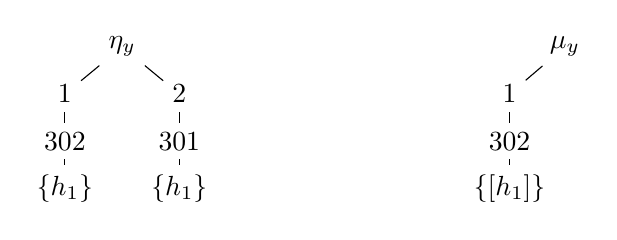
\begin{tikzpicture}[outer sep=auto, level distance=12mm, scale=0.50]
  \node[xshift = 0] {$\eta_y$}
    child[xshift = -20] {node {1}
      child {node {$302$}
        child {node {$\{h_1\}$}}}
    %  child {node {$301$}
    %    child {node {$\{\}$}}}
        }
    child[xshift = 20] {node {2}
      child {node {$301$}
        child {node {$\{h_1\}$}}}
    %  child {node {$300$}
    %    child {node {$\{\}$}}}
    };
  \node[xshift=160] {$\mu_y$}
    child {node[xshift=-20] {1}
      child {node {$302$}
        child {node {$\{[h_1]\}$}}}
    %  child {node {$301$}
    %    child {node {$\{\}$}}}
    };
    %child {node[xshift=20] {2}
    %  child {node {$301$}
    %    child {node[yshift=-2em] {$\{\}$}}}};
\end{tikzpicture}
\end{center}

The next step is to add $h_2 : 300 \leq 301$ to the maps.
Again, it unifies with both slots 1 and 2; we start by updating the map $\eta_y(1, y \mapsto 301)$ with $\{h_2\}$.
Again, an update in slot 1 causes the creation of a level 1 match.
We then check whether there are suitable hypotheses in slot 2 with
with a compatible instantiation of $y$; indeed we find $\eta_y(2, y \mapsto 301) = \{h_1\}$.
This update the match map with the level 2 match $[h_2,h_1]$.
This is a complete match.
The new hypothesis $h_3 : 300 \leq 302$ is added to the context.

The hypothesis $h_2$, also matches with slot 2.
This causes the update $\eta_y(2, y \mapsto 300)$ with $\{h_2\}$. 
At this point, we need to check for level 1 that would be compatible, there are none and the work with this hypothesis is done.

\begin{center}
    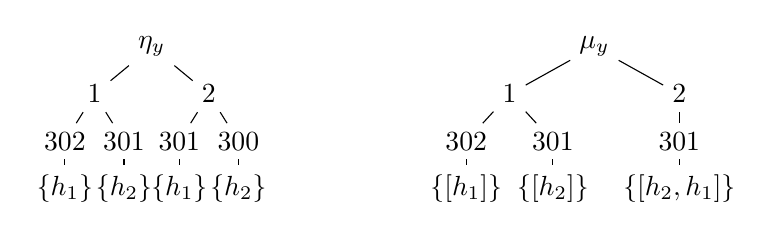
\begin{tikzpicture}[outer sep=auto, level distance=12mm, scale=0.50]
      \node[xshift = 0] {$\eta_y$}
        child[xshift = -20] {node {1}
          child {node {$302$}
            child {node {$\{h_1\}$}}}
          child {node {$301$}
            child {node {$\{h_2\}$}}}
            }
        child[xshift = 20] {node {2}
          child {node {$301$}
            child {node {$\{h_1\}$}}}
          child {node {$300$}
            child {node {$\{h_2\}$}}}
        };
      \node[xshift=160] {$\mu_y$}
        child {node[xshift=-20] {1}
          child[xshift=-10] {node {$302$}
            child {node {$\{[h_1]\}$}}}
          child[xshift=10] {node {$301$}
            child {node {$\{[h_2]\}$}}}
        }
        child {node[xshift=20] {2}
          child {node {$301$}
            child {node {$\{[h_2,h_1]\}$}}}};
    \end{tikzpicture}
    \end{center}

\paragraph{Example 2.}
We now consider another example with more than one shared variable.
Let $T_1, T_2$ be two proposition that both depend on the variable $x$ and $y$.
For simplicity, the rule considered will be $T_1(x,y) \to T_2(x,y) \to R$.
The hypotheses added to the context will be, in order, $h_1 : T_2(a,a)$, $h_2 : T_1(a,b)$ and $h_3 : T_2(a,b)$.
First, $h_1 : T_2(a,a)$ is considered :

% NOTE : remove comments to get full trees.
\begin{tikzpicture}[level distance=12mm, scale=0.50]
    \node[xshift = 30] {$\eta_x$}
        %child[xshift = -20] {node {1}
        %  child {node {$a$}
        %    child {node {$\{ \}$}}}
        %  child {node {$b$}
        %    child {node {$\{ \}$}}}}
        child[xshift = 40] {node {2}
        child {node {$a$}
            child {node {$\{h_1\}$}}}
        % child {node {$b$}
        %    child {node {$\{ \}$}}}
        };
    \node[xshift = 110] {$\eta_y$}
        %child[xshift = -20] {node {1}
        %    child {node {$a$}
        %        child {node {$\{ \}$}}}
        %    child {node {$b$}
        %        child {node {$\{ \}$}}}}
        child[xshift = 40] {node {2}
            child {node {$a$}
                child {node {$\{h_1\}$}}}
        %    child {node {$b$}
        %        child {node {$\{ \}$}}}
        };
    \node[xshift = 190, yshift = -25] {$\mu_x$};
        %child[xshift = -20] {node {1}
        %    child {node {$a$}
        %        child {node {$\{ \}$}}}
        %    child {node {$b$}
        %        child {node {$\{ \}$}}}}
        %child[xshift = 20] {node {2}
        %    child {node {$a$}
        %        child {node {$\{\}$}}}
        %    child {node {$b$}
        %        child {node {$\{ \}$}}}
        %};
    \node[xshift = 270, yshift = -25] {$\mu_y$};
        %child[xshift = -20] {node {1}
        %    child {node {$a$}
        %        child {node {$\{ \}$}}}
        %    child {node {$b$}
        %        child {node {$\{ \}$}}}}
        %child[xshift = 20] {node {2}
        %    child {node {$a$}
        %        child {node {$\{\}$}}}
        %    child {node {$b$}
        %        child {node {$\{ \}$}}}
        %};
\end{tikzpicture}

At this point, there are no matches so there is nothing to extend.
We add the next hypothesis in the queue, that is $h_2 : T_1(a,b)$, to the variable maps : 

% NOTE : uncomment to get full trees.
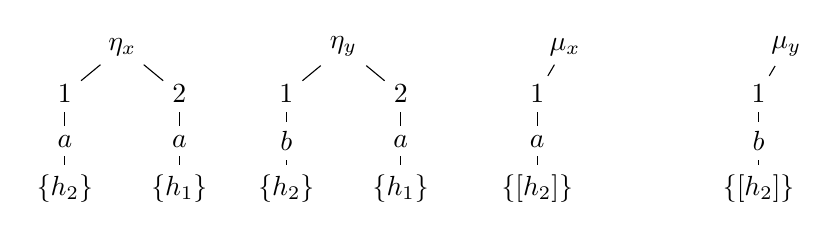
\begin{tikzpicture}[outer sep=auto, level distance=12mm, scale=0.50]
    \node[xshift = 0] {$\eta_x$}
        child[xshift = -20] {node {1}
            child {node {$a$}
                child {node {$\{h_2\}$}}}
            %child {node {$b$}
            %    child {node {$\{ \}$}}}
            }
        child[xshift = 20] {node {2}
            child {node {$a$}
                child {node {$\{h_1\}$}}}
            %child {node {$b$}
            %    child {node {$\{ \}$}}}
            };
    \node[xshift = 80] {$\eta_y$}
        child[xshift = -20] {node {1}
            %child {node {$a$}
            %    child {node {$\{ \}$}}}
            child {node {$b$}
                child {node {$\{ h_2\}$}}}}
        child[xshift = 20] {node {2}
            child {node {$a$}
                child {node {$\{h_1\}$}}}
            %child {node {$b$}
            %    child {node {$\{ \}$}}}
                };
    \node[xshift = 160, yshift = 0] {$\mu_x$}
        child[xshift = -20] {node {1}
            child {node {$a$}
                child {node {$\{[h_2]\}$}}}
            %child {node {$b$}
            %   child {node {$\{ \}$}}}
                };
        %child[xshift = 20] {node {2}
        %    child {node {$a$}
        %        child {node {$\{\}$}}}
        %    child {node {$b$}
        %        child {node {$\{ \}$}}}
        %};
    \node[xshift = 240, yshift = 0] {$\mu_y$}
        child[xshift = -20] {node {1}
        %    child {node {$a$}
        %        child {node {$\{ \}$}}}
            child {node {$b$}
                child {node {$\{[h_2]\}$}}}
        };
        %child[xshift = 20] {node {2}
        %    child {node {$a$}
        %        child {node {$\{\}$}}}
        %    child {node {$b$}
        %        child {node {$\{ \}$}}}
        %};
\end{tikzpicture}

As this hypothesis is in the first slot, we create the corresponding level 1 partial match $m_0 = {(h_2 : T_1(x, y))}$ for which we check for suitable hypotheses that could extend the match.
Note that  $s(lvl(m_0) + 1) = s(2)$ which is the intersection of the variables appearing in the slots $i < 2$ with the variables appearing in slot $2$.
Thus $s(2) = \{x,y\}$ and we compute:
\[
  \bigcap_{x\in s(lvl(m_0) + 1)} \eta_x \left(i + 1, \sigma_{m_0}(x)\right) = \eta_x(2, a) \cap \eta_y(2, b) = \emptyset
\]
Since the set is empty, the match can not be currently extended.
We turn to the remaining hypothesis $h_3 : T_2(a,b)$ in the queue and add it to the maps:

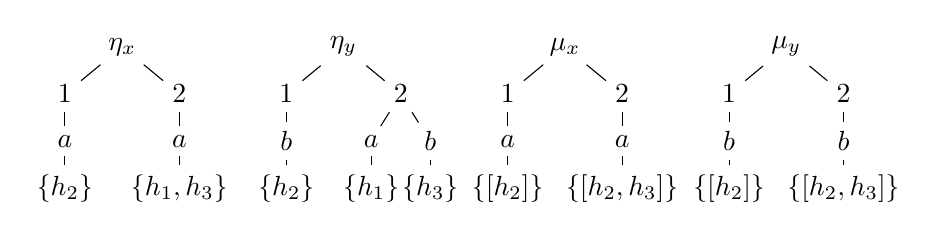
\begin{tikzpicture}[outer sep=auto, level distance=12mm, scale=0.50]
\node[xshift = 0] {$\eta_x$}
    child[xshift = -20] {node {1}
        child {node {$a$}
            child {node {$\{h_2\}$}}}
        %child {node {$b$}
        %    child {node {$\{ \}$}}}
        }
    child[xshift = 20] {node {2}
        child {node {$a$}
            child {node {$\{h_1, h_3\}$}}}
        %child {node {$b$}
        %    child {node {$\{ \}$}}}
        };
\node[xshift = 80] {$\eta_y$}
    child[xshift = -20] {node {1}
        %child {node {$a$}
        %    child {node {$\{ \}$}}}
        child {node {$b$}
            child {node {$\{h_2\}$}}}}
    child[xshift = 20] {node {2}
        child {node {$a$}
            child {node {$\{h_1\}$}}}
        child {node {$b$}
            child {node {$\{h_3\}$}}}};
    \node[xshift = 160, yshift = 0] {$\mu_x$}
        child[xshift = -20] {node {1}
            child {node {$a$}
                child {node {$\{[h_2]\}$}}}
            %child {node {$b$}
            %   child {node {$\{ \}$}}}
                }
        child[xshift = 20] {node {2}
            child {node {$a$}
                child {node {$\{[h_2,h_3]\}$}}}
        %    child {node {$b$}
        %        child {node {$\{ \}$}}}
        };
    \node[xshift = 240, yshift = 0] {$\mu_y$}
        child[xshift = -20] {node {1}
        %    child {node {$a$}
        %        child {node {$\{ \}$}}}
            child {node {$b$}
                child {node {$\{[h_2]\}$}}}
        }
        child[xshift = 20] {node {2}
        %    child {node {$a$}
        %        child {node {$\{\}$}}}
            child {node {$b$}
                child {node {$\{[h_2,h_3]\}$}}}
        };
\end{tikzpicture}

We are now ready to look for potential matches that could be extended by $h_3$.
In this particular case, since $h_3$ is in slot $2$ we look for $s(2) = \{x,y\}$.
Then,
\[
\bigcap_{x\in s(2)} \mu_x \left(i - 1, \sigma_h(x)\right) = \mu_x(1, a) \cap \mu_y(1, b) = \{m_0\}
\]

We have found two compatible hypotheses for our rule and we can then add the result $R$ as hypothesis to the context.

\jcom{TODO: deletion}

\section{Implementation}

Implementing the preceding technique efficiently requires some care, particularly in the context of dependent type theory.
We briefly discuss the most prominent challenges.

\subsection{Unification}%
\label{sec:unification}

In Lean's type theory, types contain programs and unification is expected to respect definitional equality, i.e.\ equality up to evaluation.
For instance, a theorem with premise $P~2$, where $P$ is some predicate, should apply to a hypothesis of type $P~((\Lam{x}{x})~2)$ since the two types are definitionally equal.
As a result, unifying premises and hypotheses is arbitrarily expensive in theory and a major cost centre in practice.
Our technique therefore seeks to minimise the number of unifications performed.

To limit the expense of unification, we perform unification at \emph{reducible} transparency.
Lean has multiple transparency levels that determine which constants are unfolded.
\enquote{Reducible} is the most restrictive of these, so we unfold few (and, in practice, only non-recursive) definitions, which greatly reduces the cost of unification.
It also limits the power of forward reasoning since

We also need to account for higher-order unification problems: $Q~\mvar{f}$, where $Q$ is a predicate over functions and $\mvar{f}$ is a function variable, should unify with $Q~(\Lam{x}{x})$.
Since higher-order unification is undecidable and does not admit most general unifiers (TODO ref), we use instead a unification algorithm provided by Lean that is complete for first-order unification problems and heuristically solves some higher-order problems as well.
This makes our technique incomplete in the sense that some theorem instantiations will be missed, but since the same unification algorithm is used throughout Lean, users are at least well-acquainted with this source of incompleteness.

\subsection{Data Representation}

Since the maps $μ_{x}$  and $η_{x}$ have the same domain, we may combine them into one map.
This core data structure is then represented by nested persistent hash maps: a first hash map maps variables to a second hash map, the second hash map maps slots to a third hash map and the third hash map maps instantiations to a set of hypotheses and a set of partial matches.

When we compare instantiations, the comparison should be up to definitional equality.
For example, when we try to apply a theorem $\All{x}{P~x → Q~x → R~x}$ where the first slot matches a hypothesis of type $P~a$ and the second slot matches a hypothesis of type $P~((\Lam{x}{x})~a)$, the application should succeed even though the instantiations of $\mvar{x}$ are different.
We therefore do not store $a$ and $(\Lam{x}{x})~a$ in the variable maps as-is.

Instead, we bring all instantiations into a normal form which we call \emph{reducible proof-irrelevant normal form} (RPINF).
This is the usual normal form of expressions with respect to Lean's notion of computation, except for two modifications:
\begin{itemize}
  \item Only \emph{reducible} defined constants are unfolded, i.e.\ replaced with their definiendum.
        This reflects our choice to perform unification at reducible transparency.
  \item Parts of the original expression that are proofs (in the sense that their types are members of the universe $\Prop$ of propositions) are not normalised.
        This reflects the fact that Lean's type theory definitionally equates any two proofs of the same proposition, so there is no need to check whether they are equal.
        When computing the RPINF, we also mark all proofs occurring in it with some special \enquote{metadata}.
\end{itemize}

With this setup, two expressions $t$ and $u$ are definitionally equal at reducible transparency if their RPINFs, $t'$ and $u'$, are syntactically equal except for those portions of $t'$ and $u'$ that are proofs, which are always considered equal.
Since this is an entirely syntactic notion of equality, it can be checked very quickly and we can define an effective hash function that is compatible with it.
This allows us to use a hash map for the instantiations while still comparing them up to definitional equality.

We believe that this scheme is more efficient than alternative schemes relying on repeated unification.
For example, we could use Lean's implementation of imperfect discrimination trees (TODO ref), which implement a map from expressions to arbitrary data where lookup respects definitional equality.
However, since these discrimination trees are imperfect, they may return spurious lookup results, so whether a lookup result is valid must be verified by unifying the query expression with the expression that was originally stored in the discrimination tree.
We believe that repeatedly performing such unifications would be, on average, more expensive than calculating one RPINF (which can be cached) for each type in a goal.

\subsection{Goal Diffs}

\jcom{Remove this whole section as too low-level?}
In Lean, the type of hypotheses can sometimes change while the hypothesis' identifier remains the same.
This means that one needs to track the types of the hypotheses as well.
We call this tracking \textit{goal diffs}, they highlight the differences between old and updated goal states.
The reference to hypotheses which changing types get deleted from the maps and the slot.
We then add them again as a new hypothesis.

\subsection{Indexing}

\subsection{Match Redundancy}

\subsection{Hypothesis Redundancy}

\jcom{Mention here that we also use this for the naive algorithm.}

\subsection{Precompilation}

\section{Evaluation}%
\label{sec:evaluation}

Comparing the stateless and stateful approach, we can draw the following conclusions about their relative performance:

\begin{itemize}
    \item The stateful algorithm maybe be expected to perform poorly when the context contains many hypotheses that almost complete rules.
    \item The stateless algorithm should perform decently well on average and especially when only the last premises are absent, so the rules get never selected by the stateless index.
\end{itemize}


These tests were performed on a Macbook Pro with the Apple M2 Pro chip equipped with 32 Go of RAM.
The tests showcased in this section are available here \footnote{\xcom{TODO : Link Github repo with tests.}}
\subsection{Results}
\xcom{TODO: Add a comment on the effect it had on Mathlib.}

We present here a number of results obtained by running synthetic tests.
By synthetic we mean that these tests we're constructed solely for the purpose of demonstrating the different complexity behavior of both algorithms by scaling some parameter (e.g.\ the number of rules).
The results of the tests are an average of multiple runs.

\paragraph{Transitivity.}

\begin{figure}
    \label{fig:trans}
    % Transitivity with precompilation.
    % 
    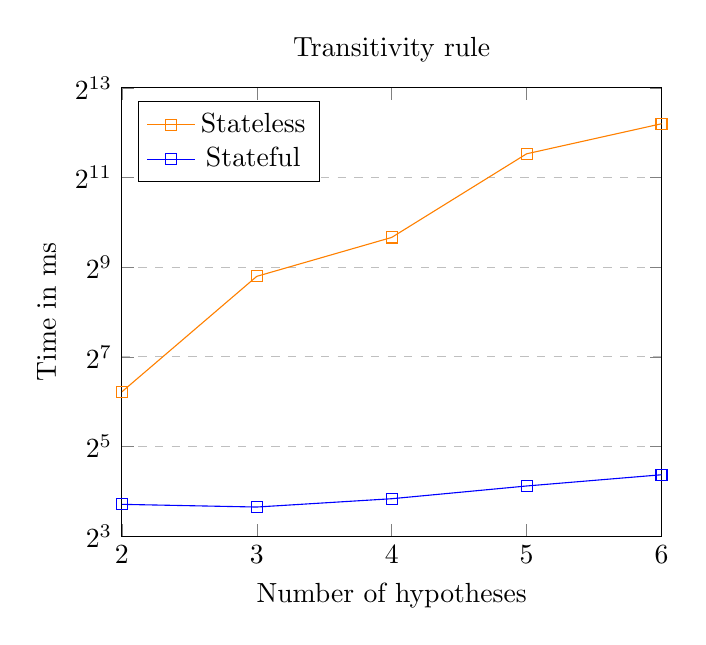
\begin{tikzpicture}
        \begin{axis}[
            title={Transitivity rule},
            xlabel={Number of hypotheses},
            ylabel={Time in ms},
            xmin=2, xmax=6,
            ymin=2^3, ymax=2^13,
            xtick={2,3,4,5,6},
            ytick={2^3,2^5,2^7,2^9,2^11,2^13},
            ymode=log,
            %xmode=log,
            log basis y=2,
            legend pos=north west,
            ymajorgrids=true,
            grid style=dashed,
        ]
        
        \addplot[
            color=orange,
            mark=square,
            ]
            coordinates {
                (2, 74.566944) (3, 444.481222) (4, 811.149916) (5, 2955.663569) (6, 4703.832541) 
            };
            \addlegendentry{Stateless}
        \addplot[
            color=blue,
            mark=square,
            ]
            coordinates {
                (2, 13.089680) (3, 12.556333) (4, 14.278986) (5, 17.385902) (6, 20.682083)
            };
            \addlegendentry{Stateful}
        \end{axis}
        \end{tikzpicture}
    \end{figure}

As a first example, which we believe highlights well the advantages of the stateful approach, we consider a scaled up version of a transitivity problem.
As variables we choose a custom version of natural numbers.
The reason being that Lean has special optimization procedures for its integer and thus makes evaluation quite hard on problems that use them; the unification is too quickly resolved, making algorithmic complexity difficultly distinguishable from noise.
We aim to emulate a more general problem where the objects unified do not benefit of some special support.

Given some predicate $P(x, y)$, we register the rule $r : P(x, y) \to P(y, z) \to P(x, z)$ to both algorithms.
Then, in Figure \ref{fig:trans}, we compare them on a context containing $n$ hypotheses of the form $(h_1 : P(a, n + 1)), \dots, (h_n : P(a + n - 1, a + n))$.
Saturating this goal adds a total of $n(n-1)/2$ hypotheses to the context.

The results in Figure \ref{fig:trans} have nothing surprising : The stateless algorithm needs to go over the whole context, which contains initially $n$ hypotheses and compares them with these same $n$ hypotheses.
This is repeated approximately for each of the $n(n-1)/2$ added hypotheses giving the expected complexity of $O(n^4)$.

The stateful algorithm considers each of the problem's hypothesis, both the initial and added ones, only once.
As the hypotheses get matched to both slots, it then compares it with at most $n$ hypotheses for each slot.
Indeed, by the end of the saturation procedure, for a value $k$ fixed, the first slot $\eta_y(1,k)$, contains at most $n$ hypotheses of the form $h : P(m,k)$ and symmetrically for the second slot.
This leaves an expected complexity of $O(n^2)$.

There are of course obvious inefficiencies, even with the stateful algorithm.
For this specific kind of problem, the hypotheses need only be used once and this leads to much repeated work.
For these scenarios, users can register the rule as a \textit{destruct} rule, eliminating hypotheses after their first use.
In this case, the complexity is linear in $n$.
For more edge case examples like this one, consult the project's repository.

\paragraph{Independent rules.}

\begin{figure}
    %Indep with precompilation
        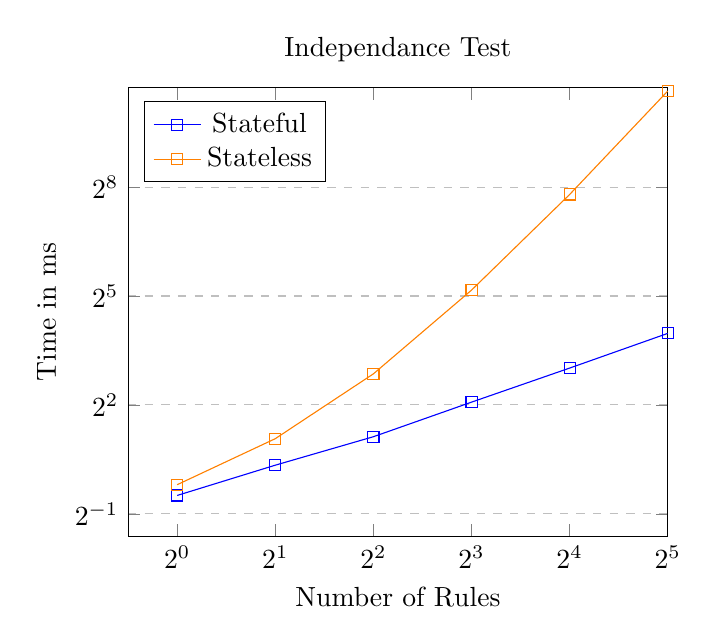
\begin{tikzpicture}
            \begin{axis}[
                title={Independance Test},
                xlabel={Number of Rules},
                ylabel={Time in ms},
                xmin=0, xmax=32,
                ymin=0, ymax=1700,
                ymode=log,xmode=log,
                log basis x=2,
                log basis y=2,
                legend pos=north west,
                ymajorgrids=true,
                grid style=dashed,
            ]
            
            \addplot[
                color=blue,
                mark=square,
                ]
                coordinates {
                (1, 0.710963)(2, 1.266787)(4, 2.181111)(8, 4.220279)(16, 8.084744)(32, 15.683840)
                };
                \addlegendentry{Stateful}
            \addplot[
                color=orange,
                mark=square,
                ]
                coordinates {
                (1, 0.872730)(2, 2.100940)(4, 7.245598)(8, 35.805959)(16, 222.283526)(32, 1600.978502)
                };
                \addlegendentry{Stateless}
            \end{axis}
            \end{tikzpicture}
        \end{figure}

In the last example, part of the stateful algorithm's success stems from the fact that it could reuse a lot of its previous work.
An obvious question is then how well does the stateful algorithm work when there is no work to be reused.

Given a set of propositions $\mathcal{P} := \{P_{i,j} | 1 \leq i \leq n \text{ and } 1 \leq j \leq 6\}$ and $\mathcal{Q} :=\{Q_{i} | 1 \leq i \leq n \}$, in this test, we consider the $n$ following rules $r_i : P_{i,1}\to \dots P_{i,6} \to Q_i$.
The procedures are then run on a context containing exactly $\mathcal{P}$.
In this case, we sketch the behavior of the stateless algorithm:
It pick a first hypothesis, $h_{i,j} : P_{i,j}$.
If $j < 6$, the index returns nothing and it selects another hypothesis.
For $h_{i,6} : P_{i,6}$, the rule $r_i$ is selected, and it then needs to try and fill its remaining five slot with the context's $6n$ hypotheses which it tries all.
This gives a complexity of about $O(n^2)$.

For the stateful algorithm, the hypotheses are considered one by one and match directly to the rule and the slot.
The expected complexity is then linear in the number of rules.

\paragraph{Depth of considered rules.}

\begin{figure}
    \label{fig:erase}
%erase with precompilation
    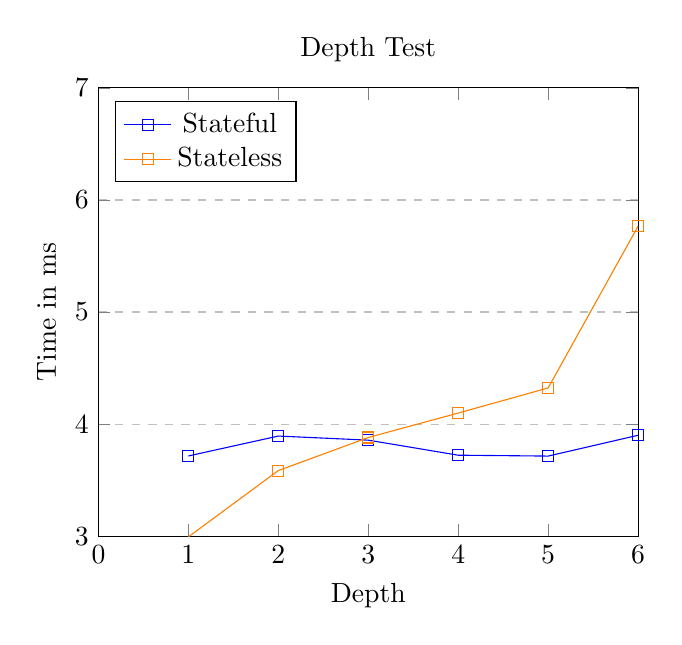
\begin{tikzpicture}
        \begin{axis}[
            title={Depth Test},
            xlabel={Depth},
            ylabel={Time in ms},
            xmin=0, xmax=6,
            ymin=3, ymax=7,
            xtick={0,1,2,3,4,5,6},
            ytick={3,4,5,6,7},
            legend pos=north west,
            ymajorgrids=true,
            grid style=dashed,
        ]
        
        \addplot[
            color=blue,
            mark=square,
            ]
            coordinates {
            (1, 3.715813)(2, 3.893547)(3, 3.856956)(4, 3.722684)(5, 3.714804)(6, 3.900508)
            };
            \addlegendentry{Stateful}
        \addplot[
            color=orange,
            mark=square,
            ]
            coordinates {
            (1, 2.993757)(2, 3.585232)(3, 3.880661)(4, 4.098640)(5, 4.322570)(6, 5.765420)
            };
            \addlegendentry{Stateless}
        \end{axis}
        \end{tikzpicture}
    \end{figure}

In Fig.~\ref{fig:erase}, the step is set up as follows: given some rule $r$ with $6$ \xcom{motivate 6} premises, we run the procedure in a context with 5 of the 6 premises present.
The numbers on the $x$ axis represent which hypothesis is missing in the order of consideration by the algorithm.
In a sense, this is how \textit{deep} the algorithm investigate before it stops.
At $0$, the rule are not selected by the index so the procedure stops.
The stateless algorithm gets progressively slower the further the removed premises is located.

The position of the missing premise has little effect on the stateful algorithm as the index selects the rule in all case; it only needs one of the premise to be present.
The work the stateful algorithm has to do is thus close to constant in this scenario.

\section{Related Work}

\paragraph{ACL2.}
Among white-box proof automation tactics, only ACL2's \enquote{waterfall} (TODO ref) has special support for forward reasoning.
(Some such tactics, e.g.\ Coq's \texttt{auto}, can execute arbitrary tactics including forward rules, but make no special provisions for them.)
Like Aesop, ACL2 works on goals and saturates the local context of each goal, using user-provided forward rules, before using backward reasoning proof methods.
It uses essentially Aesop's naive algorithm, i.e.\ the local context of each goal is saturated independently without reusing partial results from other goals.

\paragraph{SATCHMO.}
The Prolog-based first-order theorem prover SATCHMO (TODO ref) and its many descendants (TODO refs) uses a tableau calculus (TODO ref) that can be viewed as combined forward and backward reasoning.
Given a set of implications $A₁ ∧ \dots ∧ Aₙ → B₁ ∨ \dots ∨ Bₘ$ (with special cases $⊤ → B₁ ∨ \dots ∨ Bₘ$ and $A₁ ∧ \dots ∧ Aₙ → ⊥$), SATCHMO attempts to create a model that satisfies all implications.
To that end, it matches the premises $A₁, \dots, Aₙ$ of each rule against known facts from Prolog's database, which is initially empty.
If this is successful, SATCHMO first adds $B₁$ to the Prolog database and continues its search; if the continuation fails (i.e., if $⊥$ is derived), SATCHMO backtracks and tries $B₂$, etc.

This search procedure can be viewed as a special case of our technique: the implications are used as forward rules and a single backward rule splits any goal with target $B₁ ∨ \dots ∨ Bₘ$ into $m$ goals with targets $B₁, \dots, Bₘ$.
Compared to a Prolog-based implementation, our technique has the advantage that at each branching point we remember the partial matches induced by the currently known facts for each implication, rather than matching the implication against the database multiple times (subject to one of Prolog's various indexing schemes).
Whether this gain outweighs the cost of storing and maintaining the partial match data structures likely depends on the given implications.
Another advantage is that our technique is agnostic to the search strategy, whereas SATCHMO's Prolog implementation is based on backtracking and hence must use depth-first search.

\paragraph{Knowledge-based reasoning systems.}
Combined forward and backward reasoning is also supported by some knowledge-based reasoning systems, e.g.\ Algernon (TODO ref) and EYE (TODO ref).
However, to our knowledge none of these systems have backwards rules that can change the facts available to forward rules.
Hence backward and forward reasoning do not interact and there is no need for our technique.
Nevertheless, our proposal bears some resemblance to the RETE algorithm (TODO ref) for forward reasoning in large knowledge bases.

\paragraph{Other related work.}
More distantly related are various calculi that combine backward reasoning with some form of incremental forward reasoning or simplification.
Examples include the DPLL algorithm with its unit resolution rule (TODO ref) or incremental theory reasoners in SMT (TODO ref) and tableaux (TODO refs).
Focusing (TODO ref) provides a proof-theoretic view on the interplay of forward and backward reasoning.

\jcom{auto2}

\section{Conclusion}

\xcom{Do we want to add potential improvements? Like an index closer to the naive algorithm.}

TODO

\end{document}


% \begin{figure}
%     % This is the erase without precompilation for 6 premises.
%     % Note I have a decent idea that would allow us to compare for multiple
%     % number of premises. 
%     % (Divide by the average of the stateful time to normalize.)
%     \begin{tikzpicture}
%         \begin{axis}[
%             title={Depth Test},
%             xlabel={Depth},
%             ylabel={Time in ms},
%             xmin=0, xmax=6,
%             ymin=50, ymax=65,
%             xtick={0,1,2,3,4,5,6},
%             ytick={50,55,60,65},
%             legend pos=north west,
%             ymajorgrids=true,
%             grid style=dashed,
%         ]
        
%         \addplot[
%             color=orange,
%             mark=square,
%             ]
%             coordinates {
%             (1,50.91)(2,53.14)(3,52.91)(4,51.22)(5,55.14)(6,56.60)
%             };
%             \addlegendentry{Stateless}
    
%         \addplot[
%             color=blue,
%             mark=square,
%             ]
%             coordinates {
%             (1,56.04)(2,56.43)(3,55.58)(4,55.26)(5,54.80)(6,60.61)
%             };
%             \addlegendentry{Stateful}
        
        
            
%         \end{axis}
%         \end{tikzpicture}
%     \end{figure}
    
%     \begin{figure}
%         % This is the erase without precompilation for 6 premises.
%         % Note I have a decent idea that would allow us to compare for multiple
%         % number of premises. 
%         % (Divide by the average of the stateful time to normalize.)
%         \begin{tikzpicture}
%             \begin{axis}[
%                 title={Scaled Depth Test},
%                 xlabel={Depth},
%                 ylabel={Time in ms},
%                 xmin=0, xmax=8,
%                 ymin=0.5, ymax=2,
%                 xtick={0,1,2,3,4,5,6,7,8},
%                 ytick={0.75,1,1.25,1.5,1.75},
%                 legend pos=north west,
%                 ymajorgrids=true,
%                 grid style=dashed,
%             ]
            
%             \addplot[color=orange,mark=square,]
%                 coordinates {(0, 0.883600)(1, 1.039751)};
%                 \addlegendentry{Stateless}
%             \addplot[color=orange,mark=square,]
%                 coordinates {(0, 0.804521)(1, 1.017893)(2, 1.022493)};
%             \addplot[color=orange,mark=square,]
%                 coordinates {(0, 0.791528)(1, 1.015467)(2, 1.076267)(3, 1.159999)};
%             \addplot[color=orange,mark=square,]
%                 coordinates {(0, 0.743256)(1, 0.966436)(2, 1.058876)(3, 1.133514)(4, 1.225561)};
%             \addplot[color=orange,mark=square,]
%                 coordinates {(0, 0.770625)(1, 1.003777)(2, 1.109929)(3, 1.215171)(4, 1.305373)(5, 1.390667)};
%             \addplot[color=orange,mark=square,]
%                 coordinates {(0, 0.759093)(1, 1.016667)(2, 1.148273)(3, 1.213138)(4, 1.342795)(5, 1.442271)(6, 1.514877)};
%             \addplot[color=orange,mark=square,]
%                 coordinates {(0, 0.709965)(1, 0.971294)(2, 1.068745)(3, 1.179333)(4, 1.312798)(5, 1.424054)(6, 1.551690)(7, 1.628344)};
%             \addplot[color=orange,mark=square,]
%                 coordinates {(0, 0.728860)(1, 1.001576)(2, 1.097472)(3, 1.219259)(4, 1.366683)(5, 1.444844)(6, 1.576972)(7, 1.668693)(8, 1.815399)};
    
            
            
                
%             \end{axis}
%             \end{tikzpicture}
%         \end{figure}
    
    
    
    
%                 \begin{figure}
%                     %Casacade with precompilation
%                         \begin{tikzpicture}
%                             \begin{axis}[
%                                 title={Casacade Test},
%                                 xlabel={Number of Rules},
%                                 ylabel={Time in ms},
%                                 xmin=0, xmax=32,
%                                 ymin=0, ymax=850,
%                                 ymode=log,xmode=log,
%                                 log basis x=2,
%                                 log basis y=2,
%                                 legend pos=north west,
%                                 ymajorgrids=true,
%                                 grid style=dashed,
%                             ]
                            
%                             \addplot[
%                                 color=blue,
%                                 mark=square,
%                                 ]
%                                 coordinates {
%                                 (1, 0.393011)(2, 0.730952)(4, 1.327736)(8, 3.007961)(16, 10.173689)(32, 38.892027)
%                                 };
%                                 \addlegendentry{Stateful}
                    
%                             \addplot[
%                                 color=orange,
%                                 mark=square,
%                                 ]
%                                 coordinates {
%                                 (1, 0.464973)(2, 0.759516)(4, 1.865191)(8, 7.585588)(16, 64.374740)(32, 813.336527)
%                                 };
%                                 \addlegendentry{Stateless}
                            
                            
                                
%                             \end{axis}
%                             \end{tikzpicture}
%                         \end{figure}
    